\begingroup
\renewcommand{\baselinestretch}{1}\selectfont
% Local, reusable vector figure styles. Units are centimetres.
\tikzset{
 thesis block/.style={draw=black,line width=.65pt,align=center,inner sep=5pt,font=\sffamily\fontsize{10}{12}\selectfont},
 thesis hw/.style={thesis block,fill=black!9},
 thesis sw/.style={thesis block,fill=white},
 thesis memory/.style={thesis block,double,double distance=1pt,fill=black!3},
 thesis arrow/.style={->,>=stealth,line width=.7pt},
 thesis transfer/.style={<->,>=stealth,line width=.7pt},
 thesis note/.style={align=center,font=\sffamily\fontsize{9}{11}\selectfont,inner sep=3pt},
 thesis title/.style={thesis note,font=\sffamily\bfseries\fontsize{10}{12}\selectfont}
}

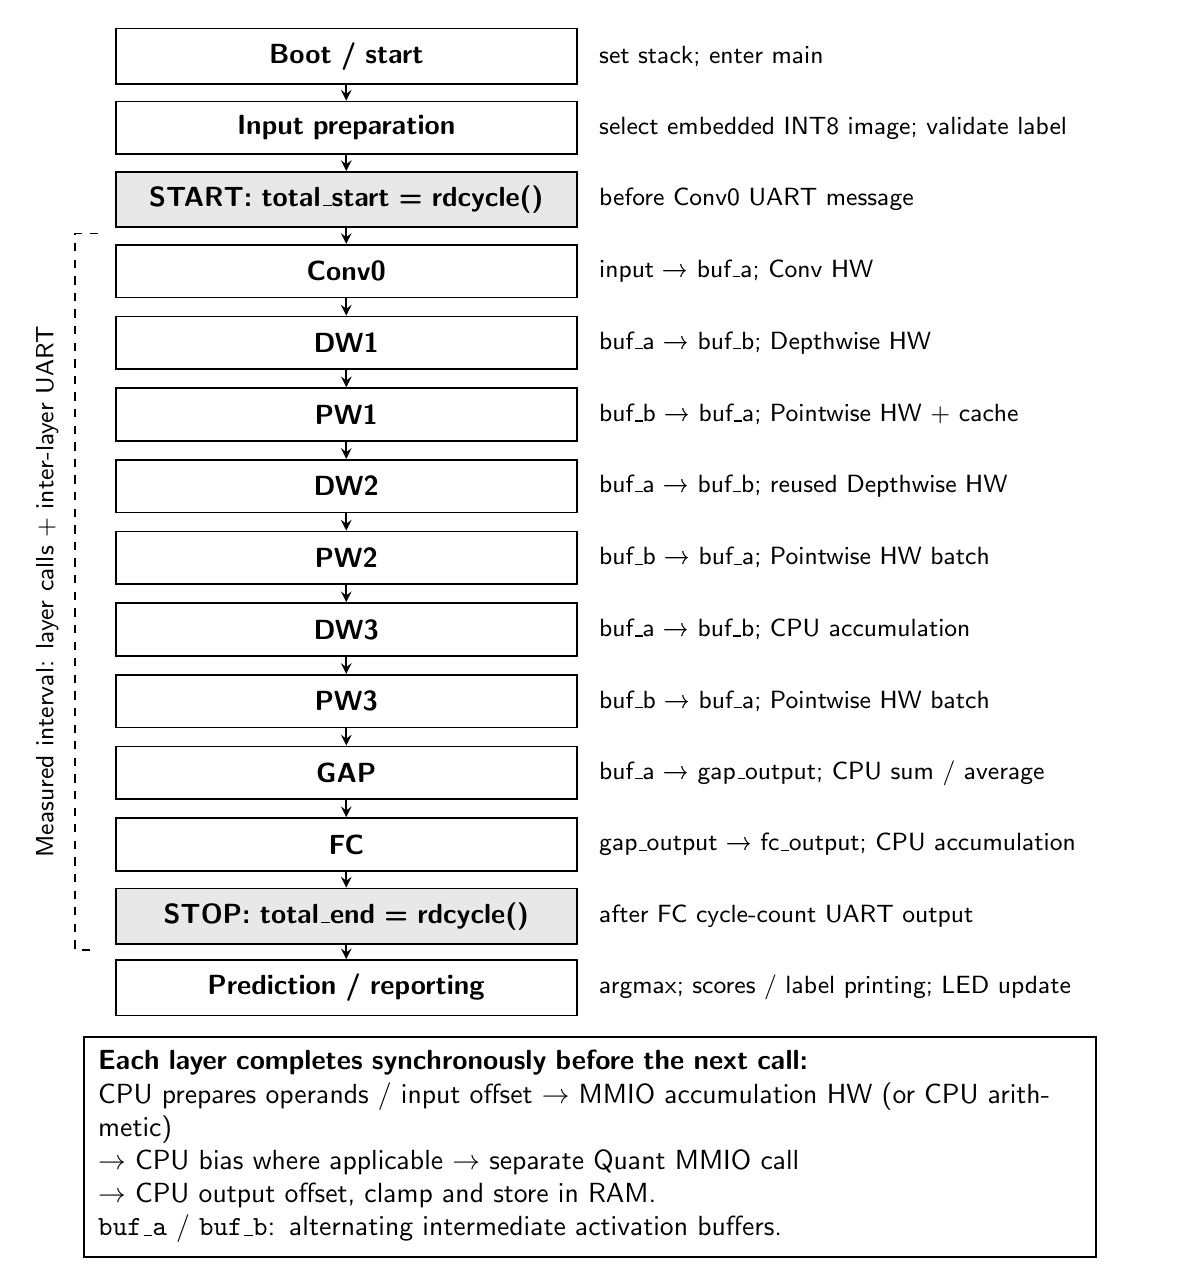
\begin{tikzpicture}[x=1cm,y=1cm]
\node[thesis sw,text width=5.5cm,minimum height=.67cm] (f0) at (3.1,0.0) {\textbf{Boot / start}};
\node[thesis note,anchor=west,align=left,text width=6.9cm] at (6.2,0.0) {set stack; enter main};
\node[thesis sw,text width=5.5cm,minimum height=.67cm] (f1) at (3.1,-0.91) {\textbf{Input preparation}};
\node[thesis note,anchor=west,align=left,text width=6.9cm] at (6.2,-0.91) {select embedded INT8 image; validate label};
\draw[thesis arrow] (f0)--(f1);
\node[thesis hw,text width=5.5cm,minimum height=.67cm] (f2) at (3.1,-1.82) {\textbf{START: total\_start = rdcycle()}};
\node[thesis note,anchor=west,align=left,text width=6.9cm] at (6.2,-1.82) {before Conv0 UART message};
\draw[thesis arrow] (f1)--(f2);
\node[thesis sw,text width=5.5cm,minimum height=.67cm] (f3) at (3.1,-2.73) {\textbf{Conv0}};
\node[thesis note,anchor=west,align=left,text width=6.9cm] at (6.2,-2.73) {input → buf\_a; Conv HW};
\draw[thesis arrow] (f2)--(f3);
\node[thesis sw,text width=5.5cm,minimum height=.67cm] (f4) at (3.1,-3.64) {\textbf{DW1}};
\node[thesis note,anchor=west,align=left,text width=6.9cm] at (6.2,-3.64) {buf\_a → buf\_b; Depthwise HW};
\draw[thesis arrow] (f3)--(f4);
\node[thesis sw,text width=5.5cm,minimum height=.67cm] (f5) at (3.1,-4.55) {\textbf{PW1}};
\node[thesis note,anchor=west,align=left,text width=6.9cm] at (6.2,-4.55) {buf\_b → buf\_a; Pointwise HW + cache};
\draw[thesis arrow] (f4)--(f5);
\node[thesis sw,text width=5.5cm,minimum height=.67cm] (f6) at (3.1,-5.46) {\textbf{DW2}};
\node[thesis note,anchor=west,align=left,text width=6.9cm] at (6.2,-5.46) {buf\_a → buf\_b; reused Depthwise HW};
\draw[thesis arrow] (f5)--(f6);
\node[thesis sw,text width=5.5cm,minimum height=.67cm] (f7) at (3.1,-6.37) {\textbf{PW2}};
\node[thesis note,anchor=west,align=left,text width=6.9cm] at (6.2,-6.37) {buf\_b → buf\_a; Pointwise HW batch};
\draw[thesis arrow] (f6)--(f7);
\node[thesis sw,text width=5.5cm,minimum height=.67cm] (f8) at (3.1,-7.28) {\textbf{DW3}};
\node[thesis note,anchor=west,align=left,text width=6.9cm] at (6.2,-7.28) {buf\_a → buf\_b; CPU accumulation};
\draw[thesis arrow] (f7)--(f8);
\node[thesis sw,text width=5.5cm,minimum height=.67cm] (f9) at (3.1,-8.19) {\textbf{PW3}};
\node[thesis note,anchor=west,align=left,text width=6.9cm] at (6.2,-8.19) {buf\_b → buf\_a; Pointwise HW batch};
\draw[thesis arrow] (f8)--(f9);
\node[thesis sw,text width=5.5cm,minimum height=.67cm] (f10) at (3.1,-9.1) {\textbf{GAP}};
\node[thesis note,anchor=west,align=left,text width=6.9cm] at (6.2,-9.1) {buf\_a → gap\_output; CPU sum / average};
\draw[thesis arrow] (f9)--(f10);
\node[thesis sw,text width=5.5cm,minimum height=.67cm] (f11) at (3.1,-10.01) {\textbf{FC}};
\node[thesis note,anchor=west,align=left,text width=6.9cm] at (6.2,-10.01) {gap\_output → fc\_output; CPU accumulation};
\draw[thesis arrow] (f10)--(f11);
\node[thesis hw,text width=5.5cm,minimum height=.67cm] (f12) at (3.1,-10.92) {\textbf{STOP: total\_end = rdcycle()}};
\node[thesis note,anchor=west,align=left,text width=6.9cm] at (6.2,-10.92) {after FC cycle-count UART output};
\draw[thesis arrow] (f11)--(f12);
\node[thesis sw,text width=5.5cm,minimum height=.67cm] (f13) at (3.1,-11.83) {\textbf{Prediction / reporting}};
\node[thesis note,anchor=west,align=left,text width=6.9cm] at (6.2,-11.83) {argmax; scores / label printing; LED update};
\draw[thesis arrow] (f12)--(f13);

\draw[dashed,line width=.65pt] (-.05,-2.25)--(-.35,-2.25)--(-.35,-11.35)--(-.05,-11.35);
\node[thesis note,rotate=90] at (-.7,-6.8) {Measured interval: layer calls + inter-layer UART};
\node[thesis block,text width=12.5cm,align=left] at (6.2,-13.85) {\textbf{Each layer completes synchronously before the next call:}\\CPU prepares operands / input offset $\rightarrow$ MMIO accumulation HW (or CPU arithmetic)\\$\rightarrow$ CPU bias where applicable $\rightarrow$ separate Quant MMIO call\\$\rightarrow$ CPU output offset, clamp and store in RAM.\\\texttt{buf\_a} / \texttt{buf\_b}: alternating intermediate activation buffers.};

\end{tikzpicture}
\endgroup
